% Generated PNG. Source: figures/gen_experiment_figs.py
% Regenerate: uv run --with matplotlib --with numpy python figures/gen_experiment_figs.py
\begin{figure}[!h]
\centering
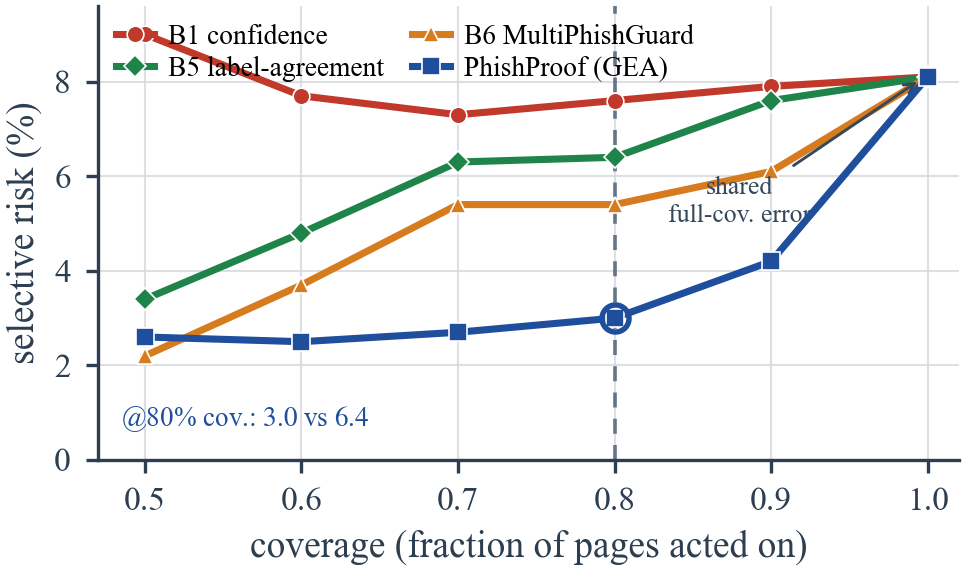
\includegraphics[width=\linewidth]{fig_riskcoverage}
\caption{Risk--coverage on \textsc{PhishSel} (RQ1, 998 pages). Lower selective risk is
better; the ring marks $80\%$ coverage. All panel methods meet at the shared
full-coverage error ($8.1\%$); \toolname{} changes only the abstention order and has
low risk as coverage tightens (best point-estimate AURC, on par with B6 within CI;
decisively the best calibration and selective accuracy).}
\Description{A line chart of selective risk versus coverage. PhishProof has the lowest
risk curve as coverage tightens and among the lowest area under the curve among the plotted
methods, which all meet at the shared full-coverage error.}
\label{fig:riskcoverage}
\end{figure}
